\documentclass[11pt,a4paper]{article}
% Locale and font
\usepackage[utf8]{inputenc}
\usepackage[T1]{fontenc}
\usepackage[english]{babel} % Set language here

% Layout
\usepackage{hyperref}
\usepackage{float}
\usepackage[margin=1cm]{caption} % Additional margin for captions
\usepackage{geometry}
\geometry{margin=1.25in} % Margin for dokument (default in Word is 1.25 inches)

\setlength{\parskip}{1em} % Skip for paragraphs
\setlength{\parindent}{0em} % Indentation for paragraphs

\usepackage[dvipsnames]{xcolor} % Color

% #########################
% Citations
\bibliographystyle{unsrt} % Set reference system here

% #########################
% Math
\usepackage{amsmath}
\usepackage{amssymb}
\usepackage{mathtools}
\usepackage{textgreek}
\usepackage{mathrsfs}

% #########################
% Physics/Chemistry
%   Chemical and nuclear reactions
%\usepackage[version=4]{mhchem} 

% Tables and plots
%   Figures
\usepackage{tikz}
\usepackage{svg}
\usepackage{graphicx}
\usepackage{subcaption}

%   Nicer tables
\usepackage{booktabs}

% #########################
% Text information
\newcommand{\Foursename}{Astrophysics 1} % Set course name here
\newcommand{\Fassignment}{Bonus Exercise} % Set assignment title here
\newcommand{\Foursecode}{\texttt{1FA204}} % Set course code here
\newcommand{\Fauthor}{Oliver Kraft} % Set author here
\newcommand{\Femail}{oliver.kraft.9720@student.uu.se} % Set email here
\newcommand{\Fersonalnumber}{20010609-XXXX}
\date{December 2021} % Set date here

%   Parameters for use in text
\title{\Foursename\, -\, \Fassignment}
\author{\Fauthor}

% #########################
% Header and footer
\usepackage{fancyhdr}

\lhead{\Foursecode}
\chead{\href{mailto:\Femail}{\texttt{\textcolor{lightgray}{\Femail}}}}
\rhead{\texttt{\Fauthor}}
\setlength{\headheight}{15pt}

\rfoot{\texttt{Page \thepage}} % Page text can be adjusted here
\lfoot{}
\cfoot{}

\fancypagestyle{plain}{
    \fancyfoot{} % Remove footer
}

\pagestyle{fancy}

% #########################
% Miscelaneous
\usepackage{pdfpages} % Include a whole pdf with \includepdf[pages=-]{file.pdf}



% Code test:
\usepackage{minted}

\begin{document}

    \begin{titlepage}
    \centering
    
\includegraphics[width=12cm]{logos/UU_logo.eps}
    \vfill
    {\bfseries\Large
    \makeatletter
    \@title\\
    \@date\\
    \vskip1cm
    \@author\\
    \vskip0.5cm
    \makeatletter
    }
    \vfill
    \vfill
\end{titlepage}
    \clearpage
    \section*{\Fassignment}

    \textbf{Note:} I'm using the following notation for labeling the plots: \texttt{[age]y[metallicity]m}.
    For instance the isochrone with stars aged $4.69 \cdot 10^9$ years with metallicity $0.0152$ would be denoted as: \texttt{4.69e9y0.0152m}.

    \begin{figure}[h]
        \centering
        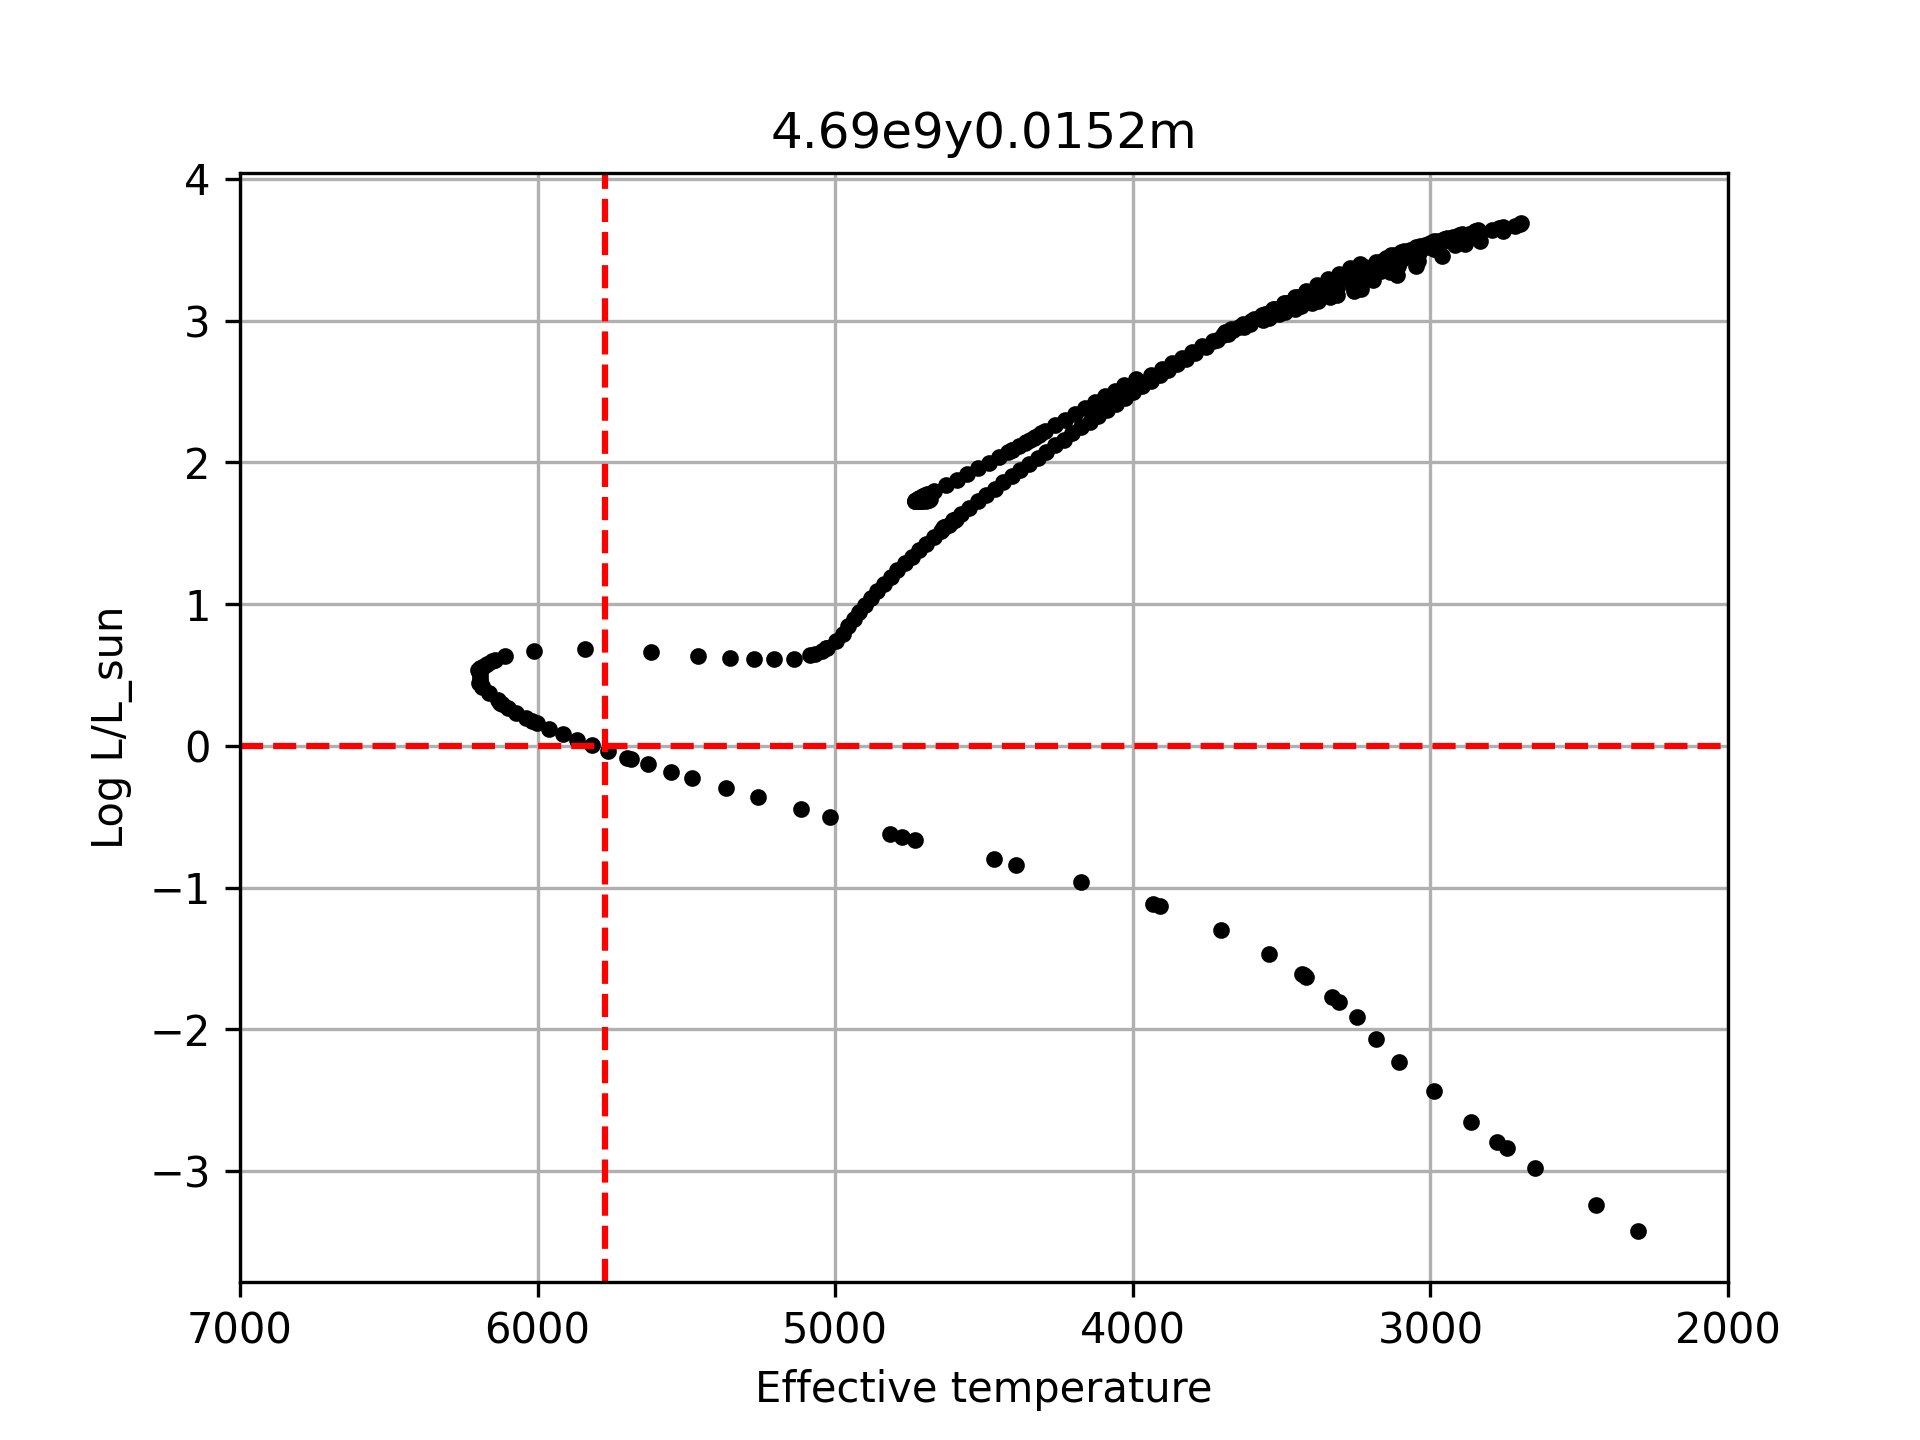
\includegraphics[width=12cm]{figures/4.69e9y0.0152m}
        \caption{HR plot of cluster with age $4.69 \cdot 10^{9}$ years and metallicity 0.0152.}
        \label{fig:ogHR}
    \end{figure}

    \textbf{1)} \textit{At which stellar initial mass, effective temperature and stellar luminosity is the turnoff point? What does this point reflect, physically?}

    Stellar initial mass: 1.69\\
    Effective temperature: approx 6200 K\\
    Luminosity: $\textrm{LogL} = 0.5 \Rightarrow L/L_{sun} = 3.16 \Rightarrow L = 1.216 \cdot 10^{27} \textrm{ W/m}^2$

    The turnoff point reflects the properties of the stars which are just about to veer off the main sequence onto the Red Giant Branch because they have expended the hydrogen in their cores.

    \textbf{2)} \textit{At which stellar initial mass, effective temperature, and stellar luminosity is the base of the Red Giant Branch?}

    Stellar initial mass: 2.45 \\
    Effective temperature: approx 6100 K ($\textrm{logTe} \approx 3.71$) \\
    Luminosity: $\textrm{LogL} = 0.575 \Rightarrow L/L_{sun} = 3.758 \Rightarrow L = 1.4461 \cdot 10^{27} \textrm{ W/m}^2$
    \newpage
    \textbf{3)} \textit{How has the appearance of the main sequence changed, compared to that shown in Fig. 1?
    What is the reason for this, in terms of nuclear fuel?}

    \begin{figure}[h]
        \centering
        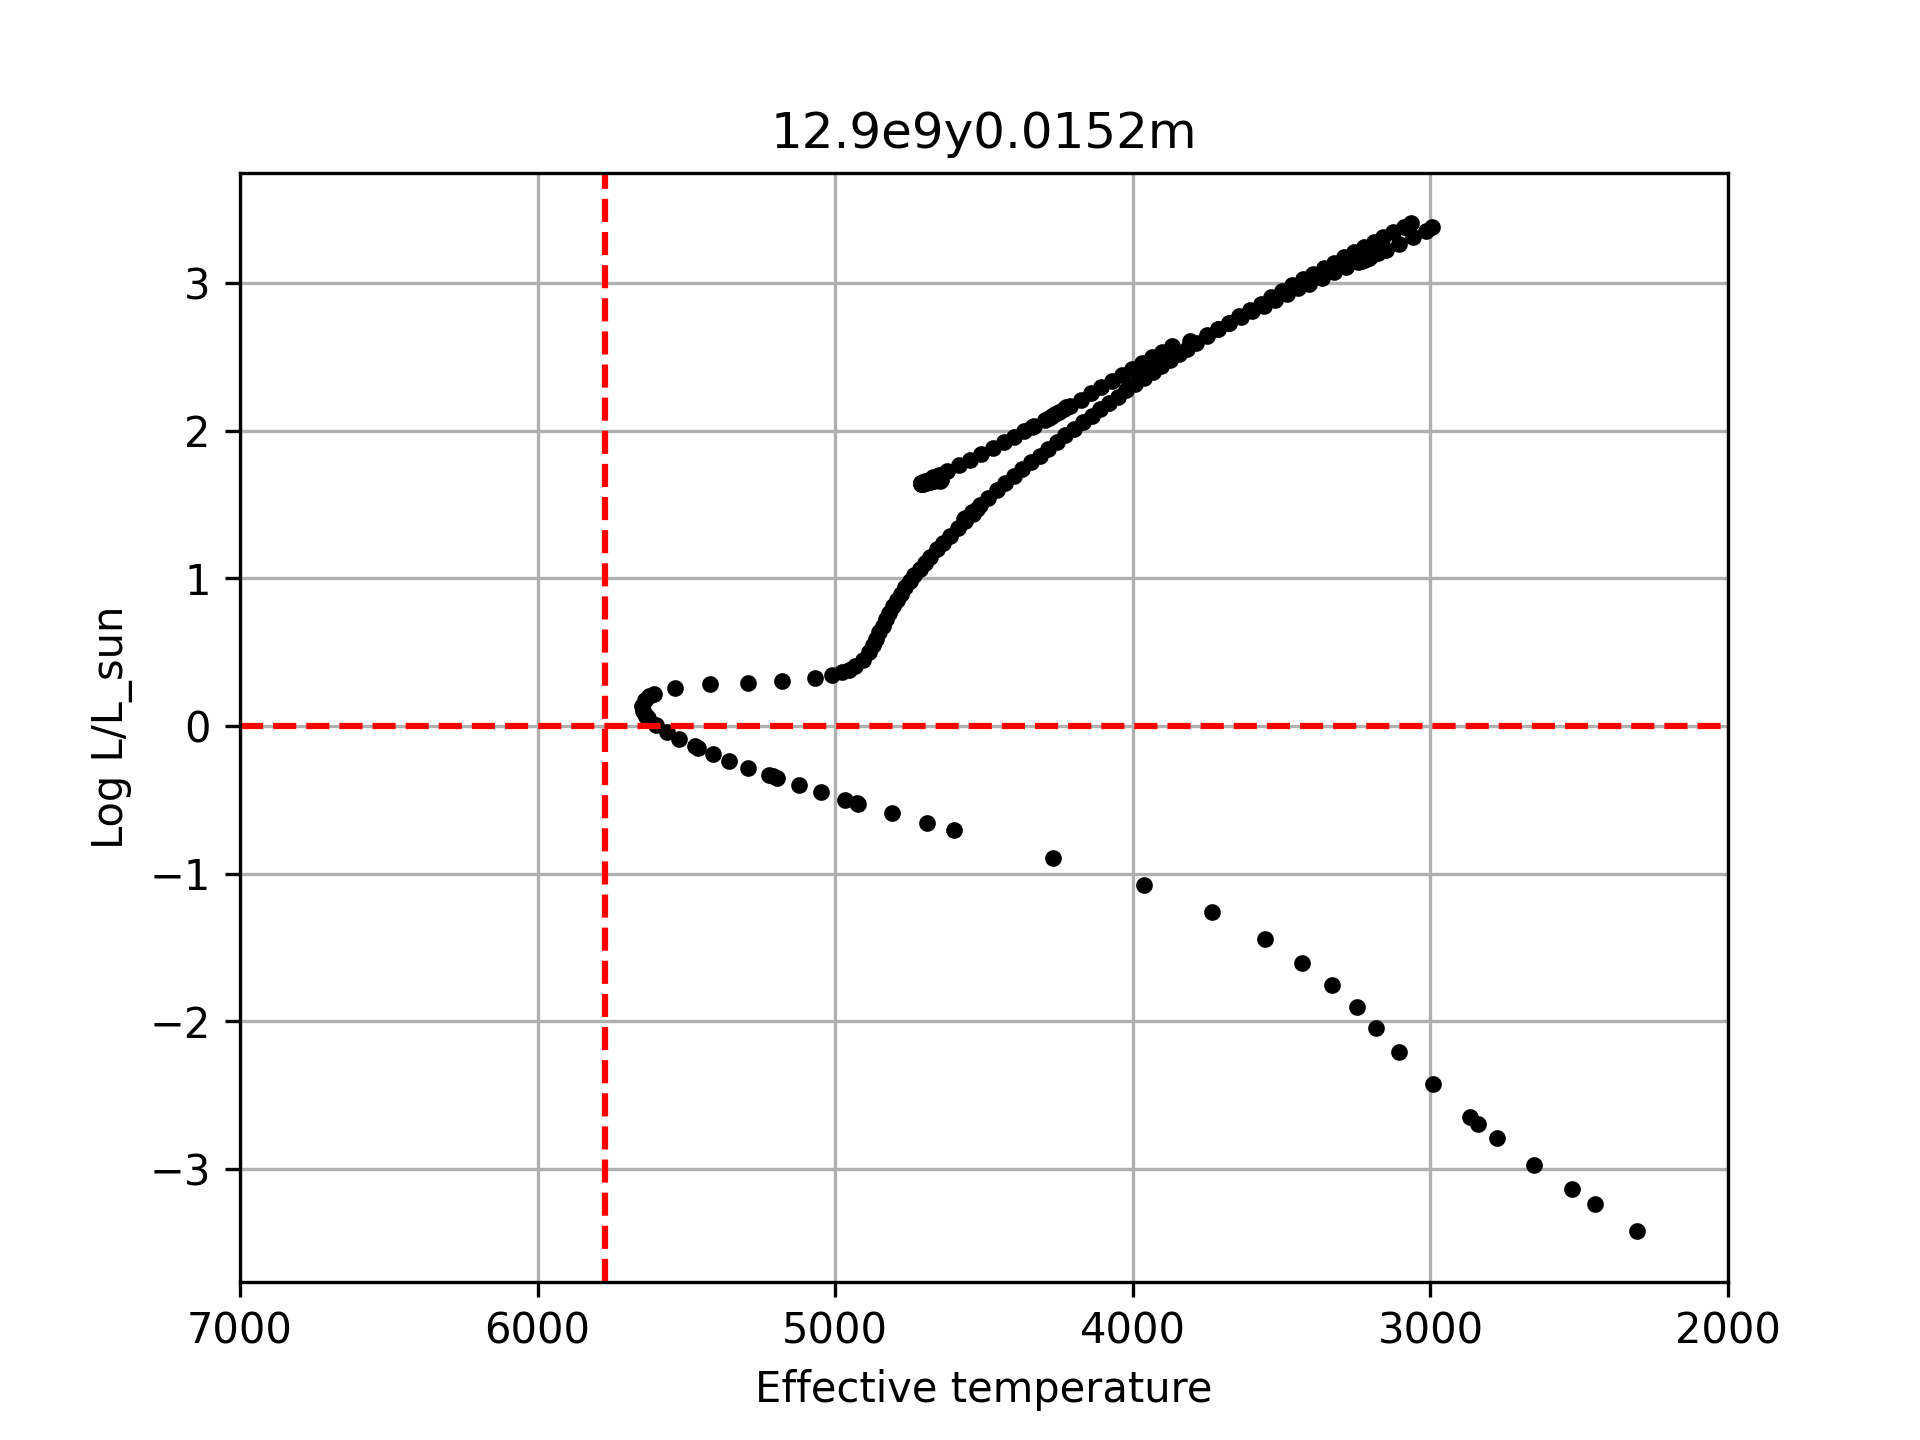
\includegraphics[width=12cm]{figures/12.9e9y0.0152m}
        \label{fig:ogHR}
    \end{figure}

    More stars have deviated from the main sequence, the turnoff point has moved down along the main sequence.
    The reason for this is that as the cluster aged more stars have had time to expend their fuel and turned onto the red giant branch.
    As the stars transition from burning hydrogen to helium the envelope will expand causing temperatures to drop.
    This causes the stars to appear redder.
    This transition will happen first for brighter stars as they expend their fuel faster and the point will thus creep downwards along the main sequence as the cluster ages.
    \newpage
    \textbf{4)} \textit{How old will the Sun be when it leaves the main sequence?
    Please estimate this by making a few more plots, varying the age of the cluster.}

    I started by plotting $11.0 \cdot 10^9$ years and $9.00 \cdot 10^9$ years.
    Then I picked an age between these two closer to 11 than 9 billion, 10.3 billion.
    Which was still a little off so I adjusted again to 10.1 billion.
    Doing this I found an age at which the sun's properties aligned very well with the turnoff point.

    The sun will leave the main sequence when it's about $10.1 \cdot 10^9$ years old.

    \begin{figure}[h]
        \centering
        \begin{subfigure}{.5\textwidth}
            \centering
            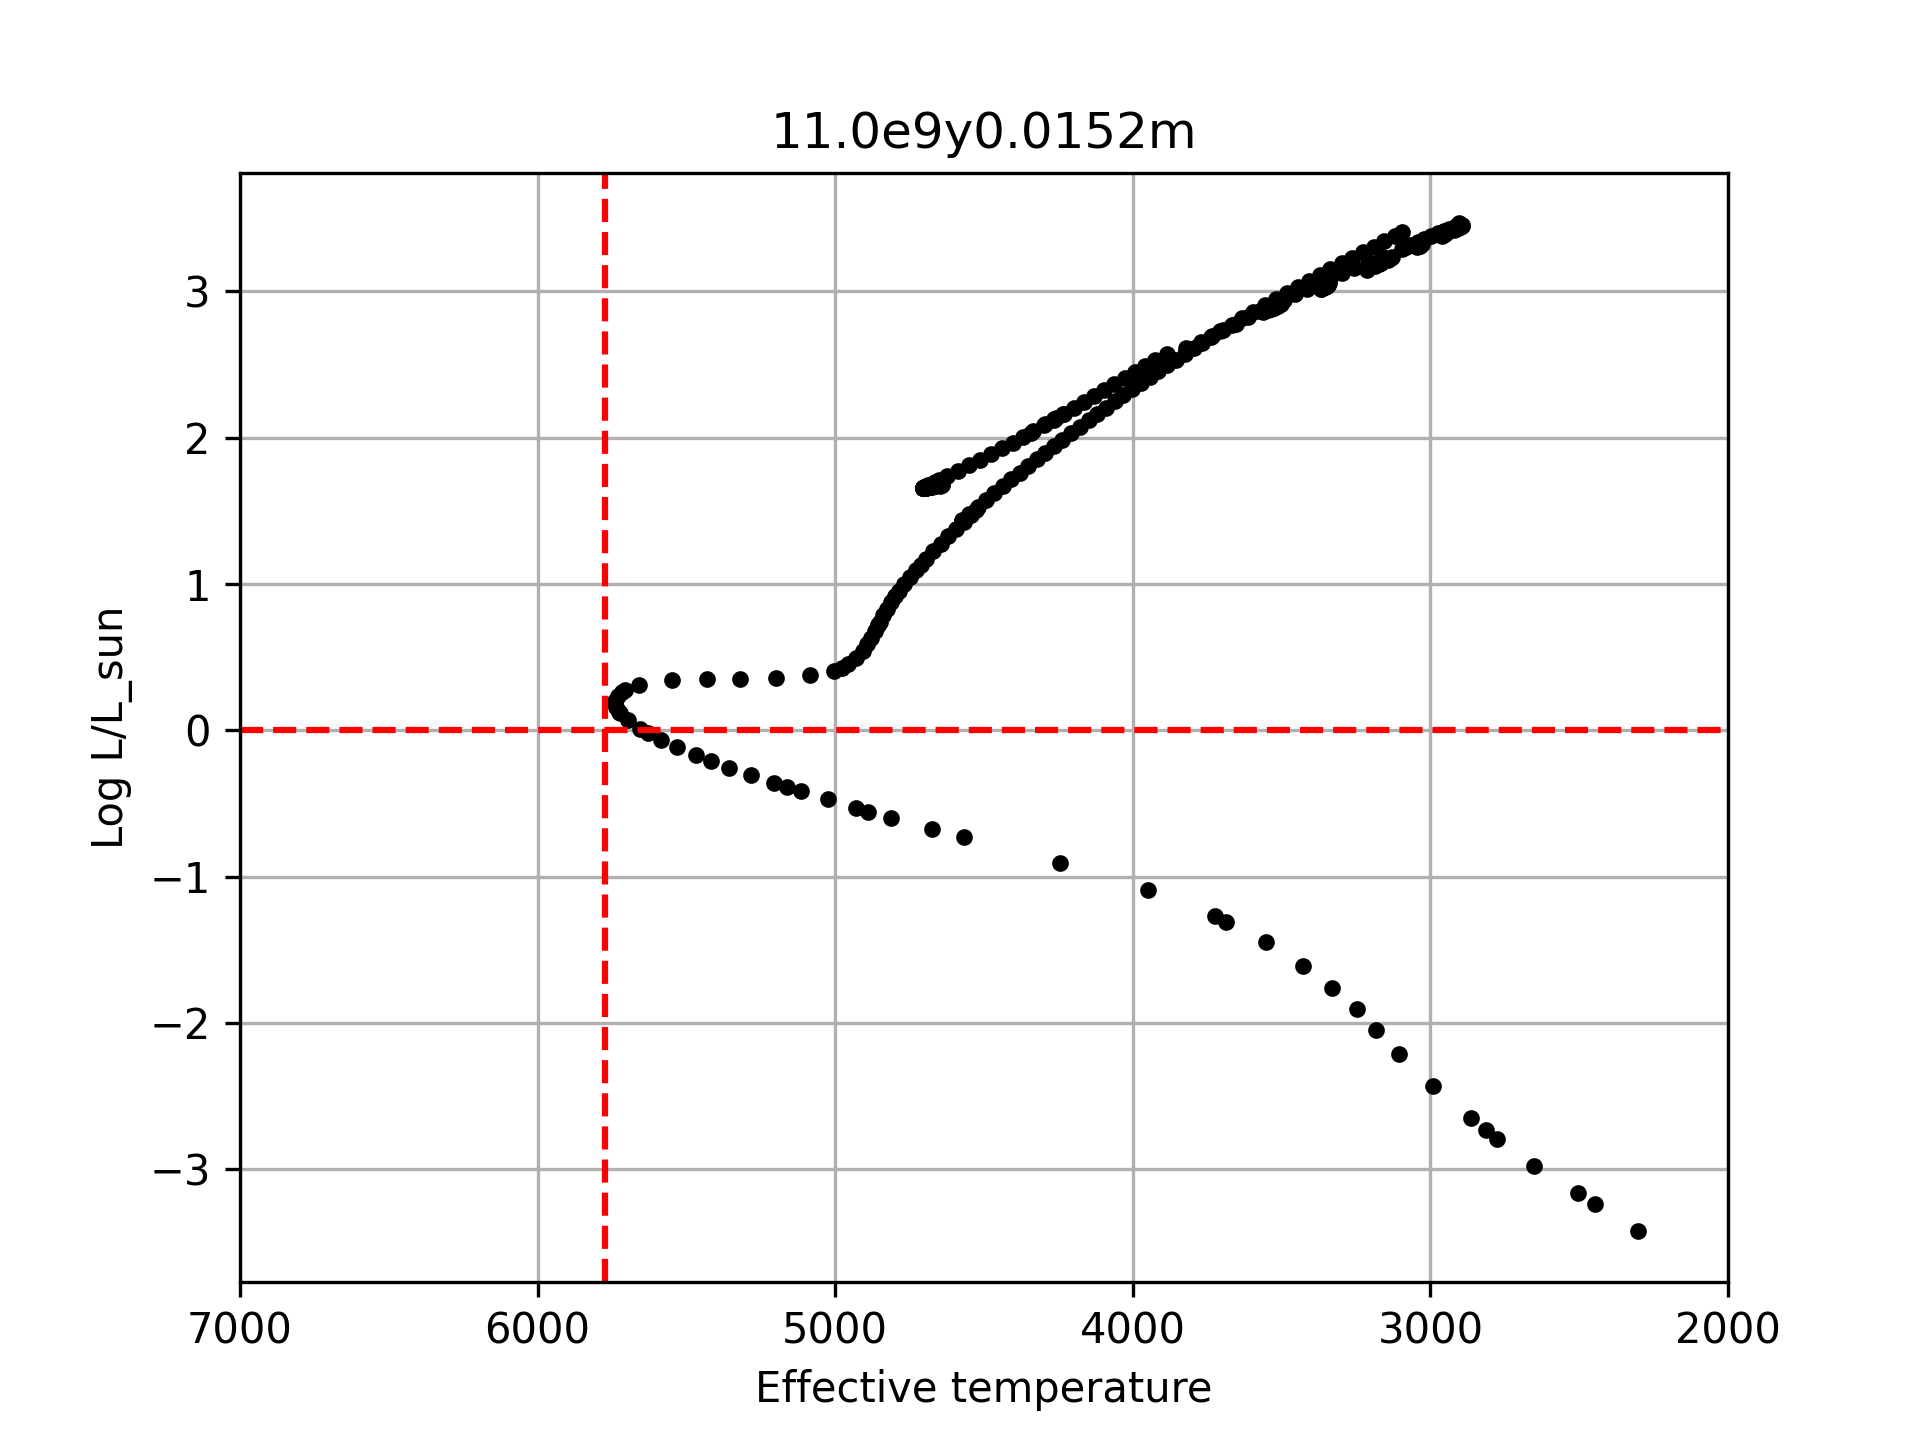
\includegraphics[width=\linewidth]{figures/11.0e9y0.0152m}
            \label{fig:sub1}
        \end{subfigure}%
        \begin{subfigure}{.5\textwidth}
            \centering
            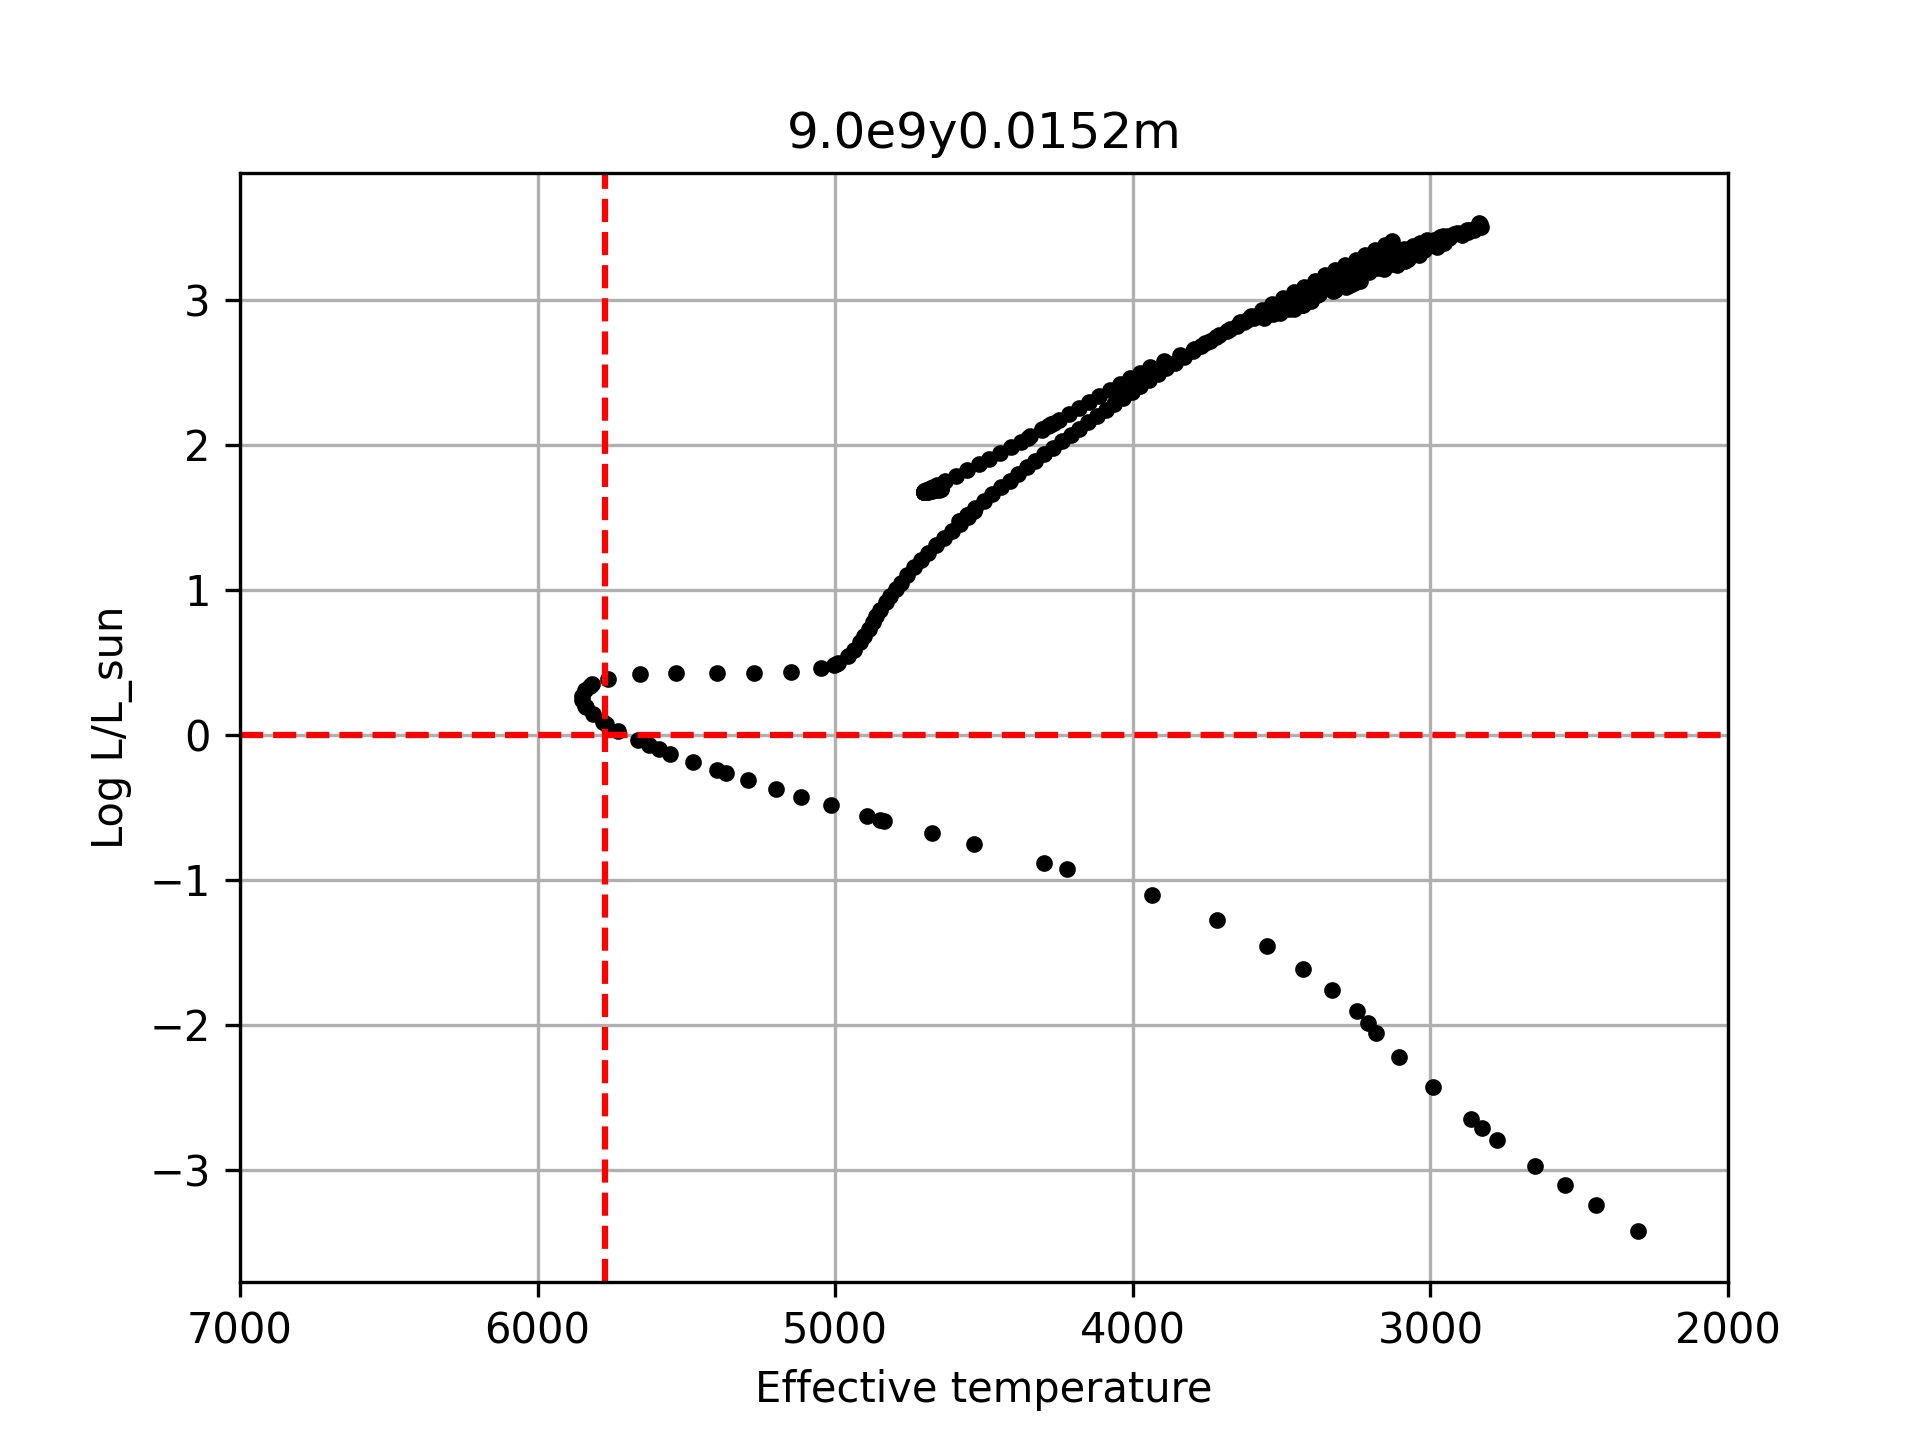
\includegraphics[width=\linewidth]{figures/9.0e9y0.0152m}
            \label{fig:sub2}
        \end{subfigure}
        \begin{subfigure}{.5\textwidth}
            \centering
            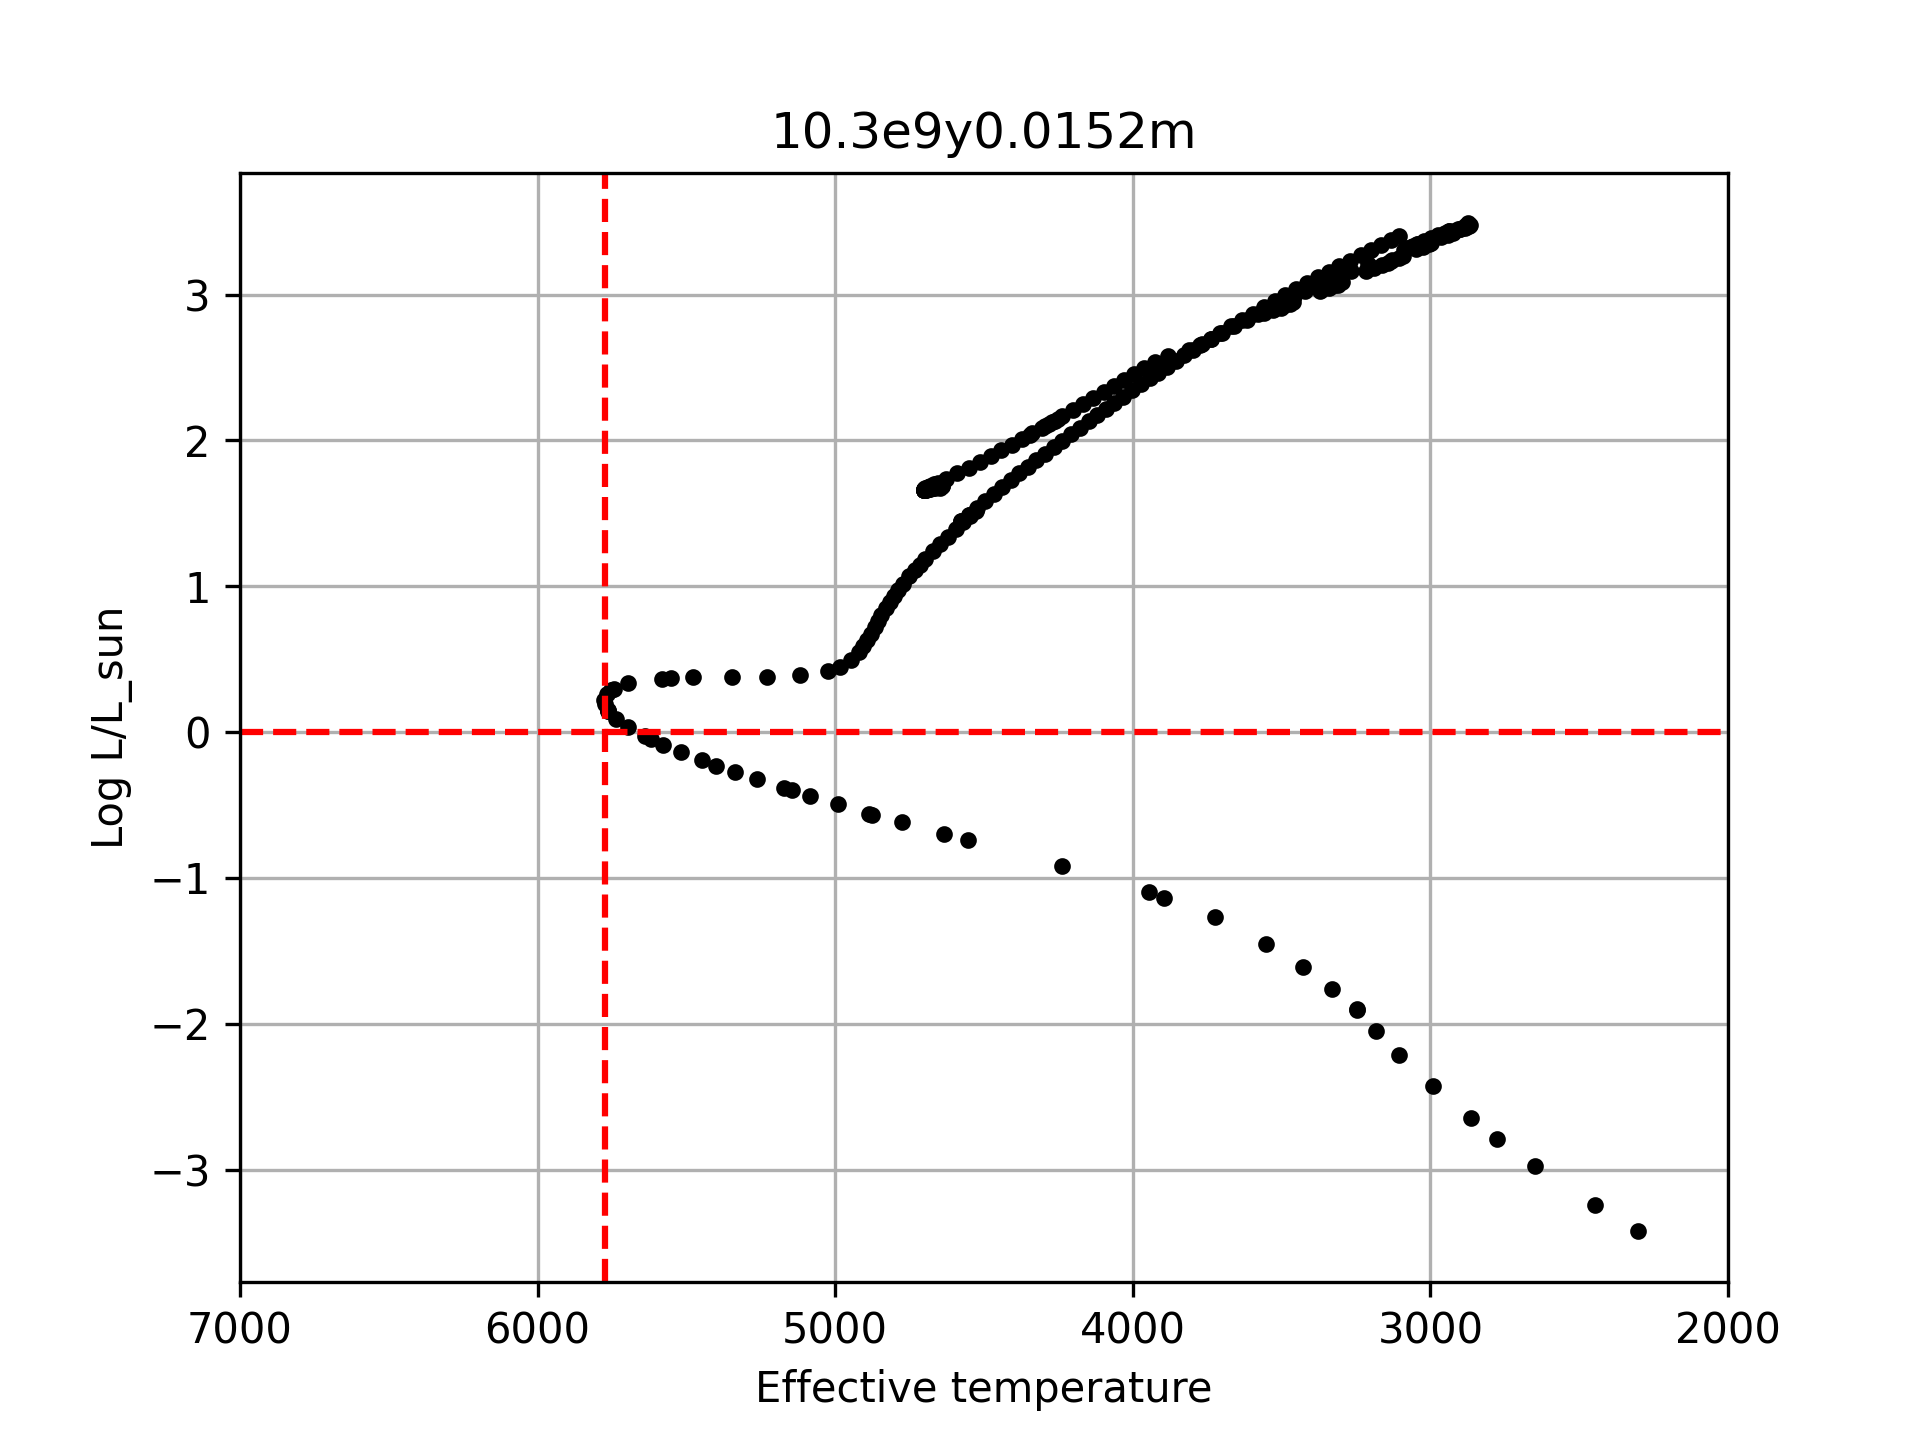
\includegraphics[width=\linewidth]{figures/10.3e9y0.0152m}
            \label{fig:sub3}
        \end{subfigure}%
        \begin{subfigure}{.5\textwidth}
            \centering
            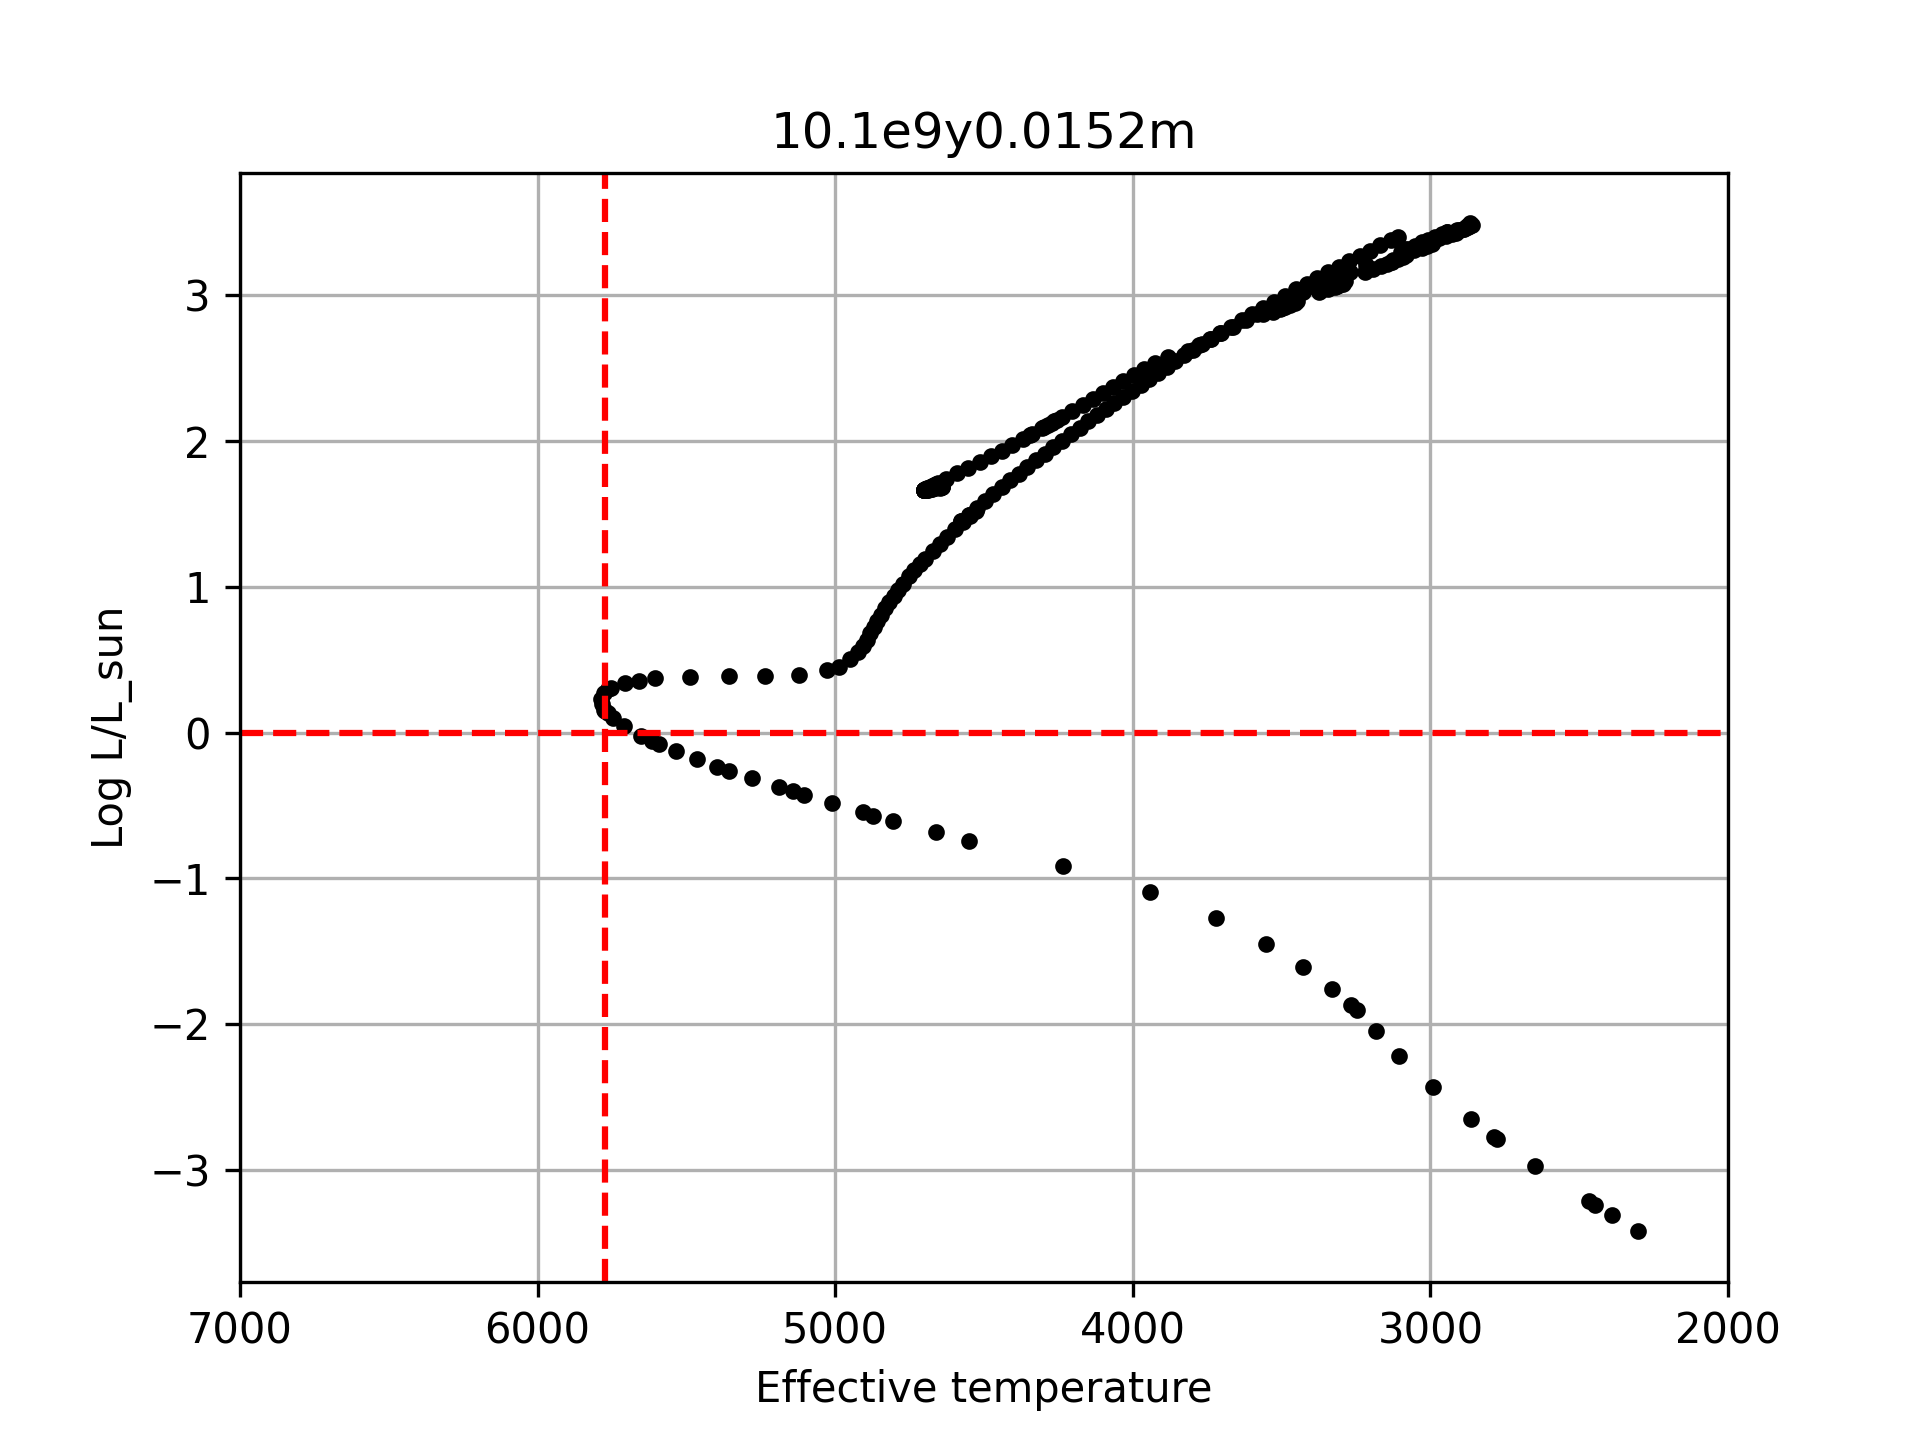
\includegraphics[width=\linewidth]{figures/10.1e9y0.0152m}
            \label{fig:sub4}
        \end{subfigure}%
        \label{fig:test}
    \end{figure}
    
    \clearpage
    
    \textbf{5)} \textit{Please attach the plot of the isochrone that corresponds to the age determined for Question 4.
    If it is not too difficult, please also show on the same figure the “standard isochrone” of 4.6 billion years and solar metallicity.}

    \begin{figure}[h]
        \centering
        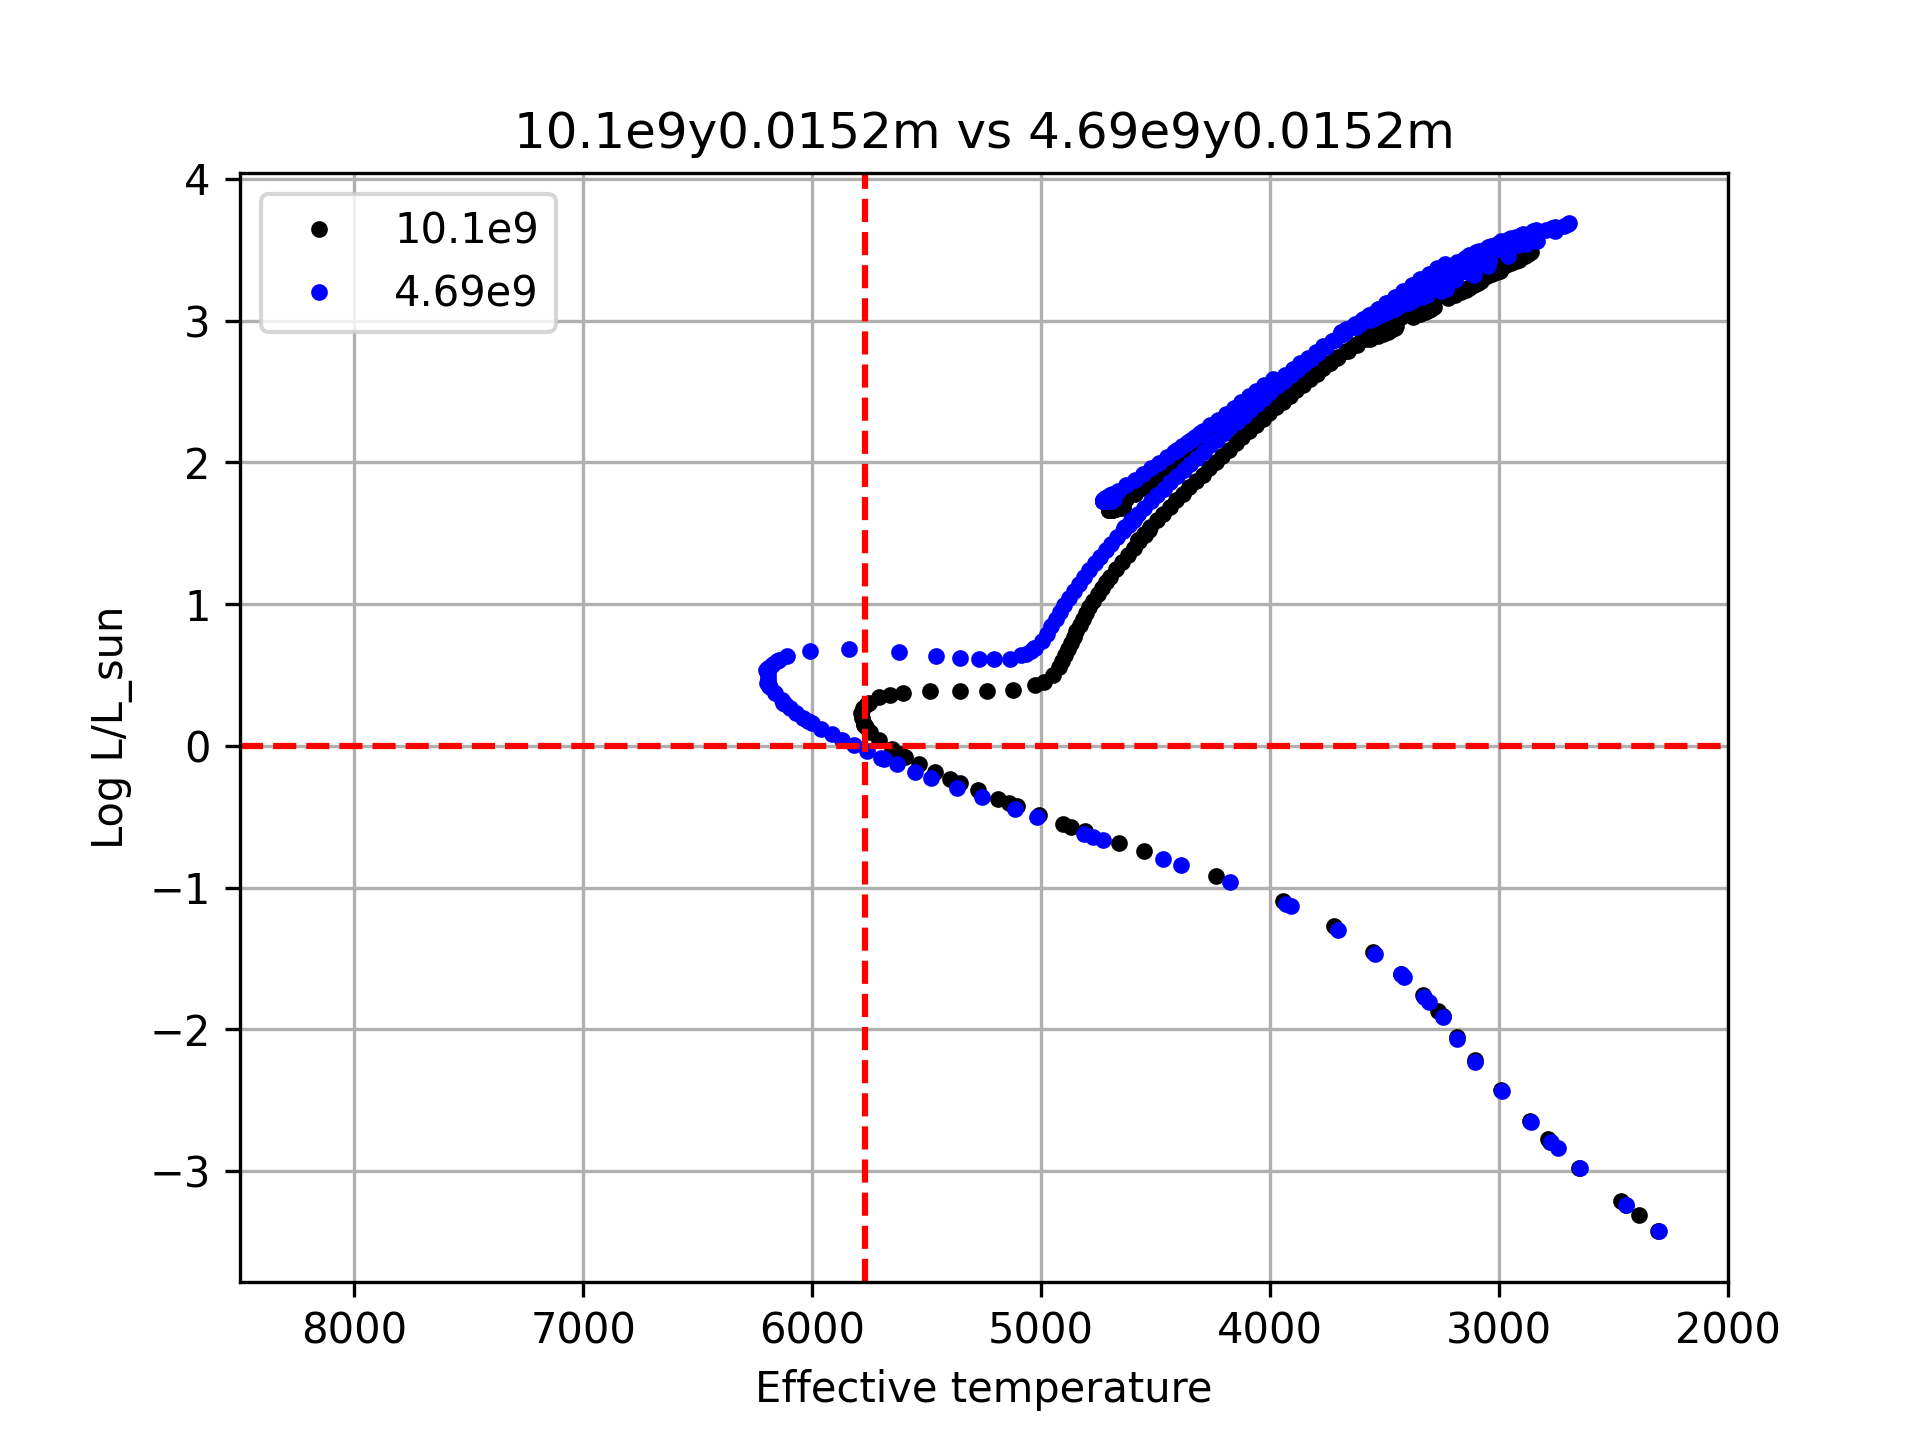
\includegraphics[width=12cm]{figures/4.69e9_vs_10.1e9y}
        \label{fig:deathOfTheSun}
    \end{figure}
    \newpage

    \textbf{6)} \textit{How has the appearance of the isochrone changed?
    Would the cluster now appear more red, more blue, or the same as before, if we were to observe it with our eyes?}

    \begin{figure}[h]
        \centering
        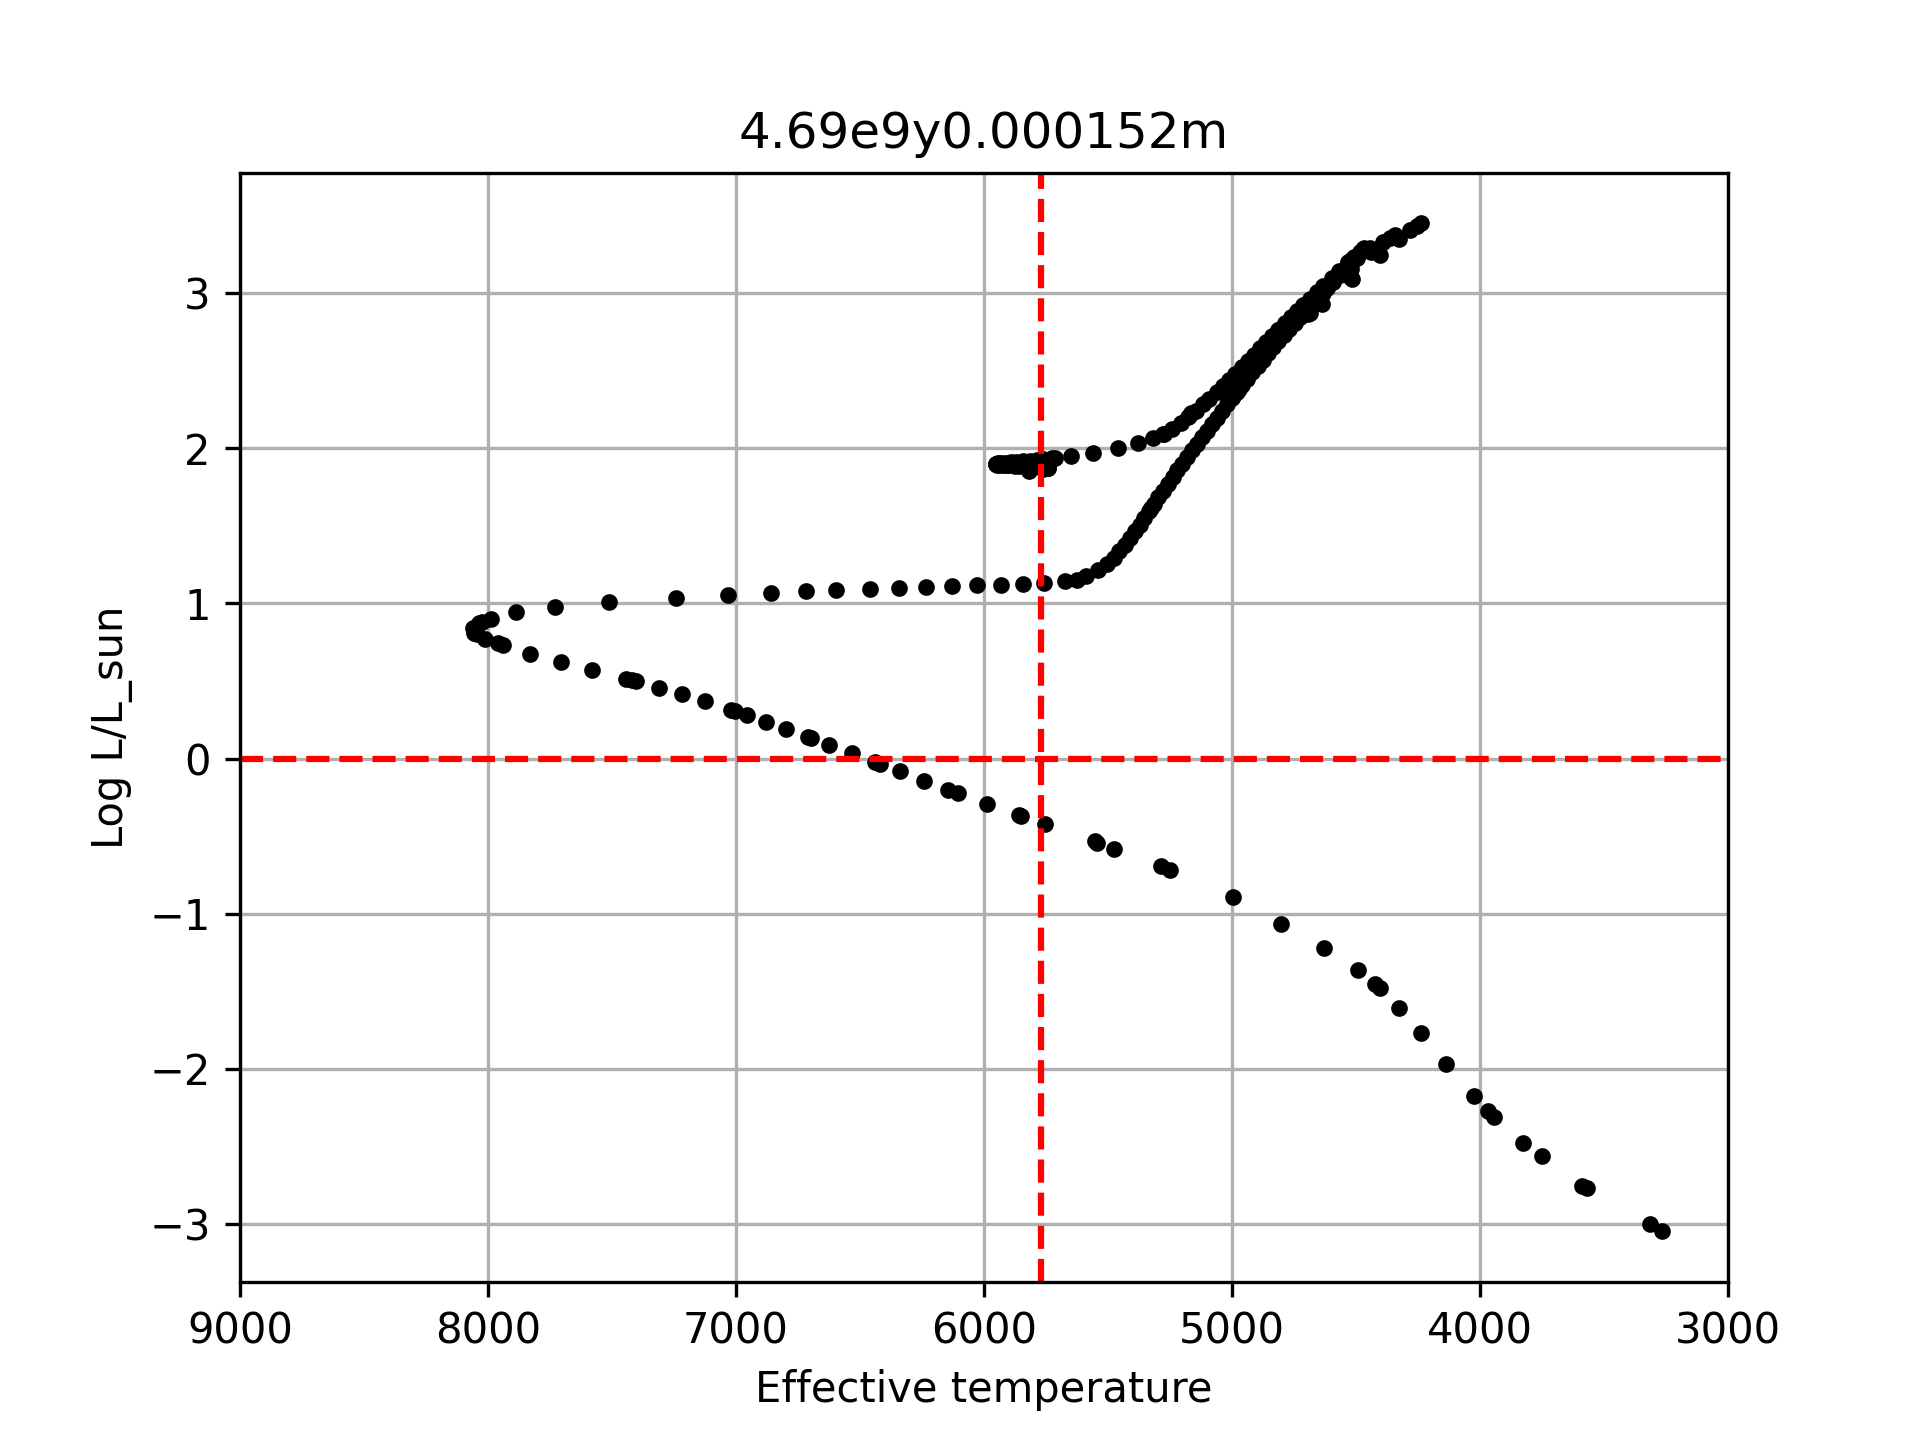
\includegraphics[width=12cm]{figures/4.69e9y0.000152m}
        \label{fig:highMetal}
    \end{figure}

    More hot stars remain on the main sequence than in the isochrone with lower metallicity, this causes the cluster to appear more blueish to our eyes.
    
    \textbf{7)} \textit{At which stellar initial mass, effective temperature and stellar luminosity is the turnoff point
    of this metal-poor cluster?
    How does this compare to the solar-metallicity cluster of the same age?}

    Stellar initial mass: 1.69\\
    Effective temperature: approx 8050 K\\
    Luminosity: $\textrm{LogL} = 0.82 \Rightarrow L/L_{sun} = 6.607 \Rightarrow L = 2.542 \cdot 10^{27} \textrm{ W/m}^2$

    Comparing to the solar-metallicity cluster of the same age it appears that the initial mass is lower for the stars at the turn off point, whilst the temperature and luminosity is higher.

    \textbf{8a)} \textit{Consider two stars with initial masses that are exactly that of the Sun, but one with
    $Z=0.0152$, and the other with $Z=0.000152$. Which of these stars spends a longer time on the main sequence? In other words, what is the impact of metallicity on the lifetime of this star?}

    At the turnoff point in the isochrone with lower metallicity the initial mass is lower than the one with higher metallicity.
    It follows that lower metallicity causes stars to expend their fuel faster.
    Thus the star with higher metallicity will spend longer on the main sequence, and will have a longer life-span.

    The star with metallicity $Z=0.0152$ will spend longer on the main sequence.

    \newpage
    \textbf{9)} \textit{Please attach a plot of the metal-poor isochrone from Question 6. If it is not too difficult,
        please also show on the same figure the “standard isochrone” of 4.6 billion years.}

    \begin{figure}[h]
        \centering
        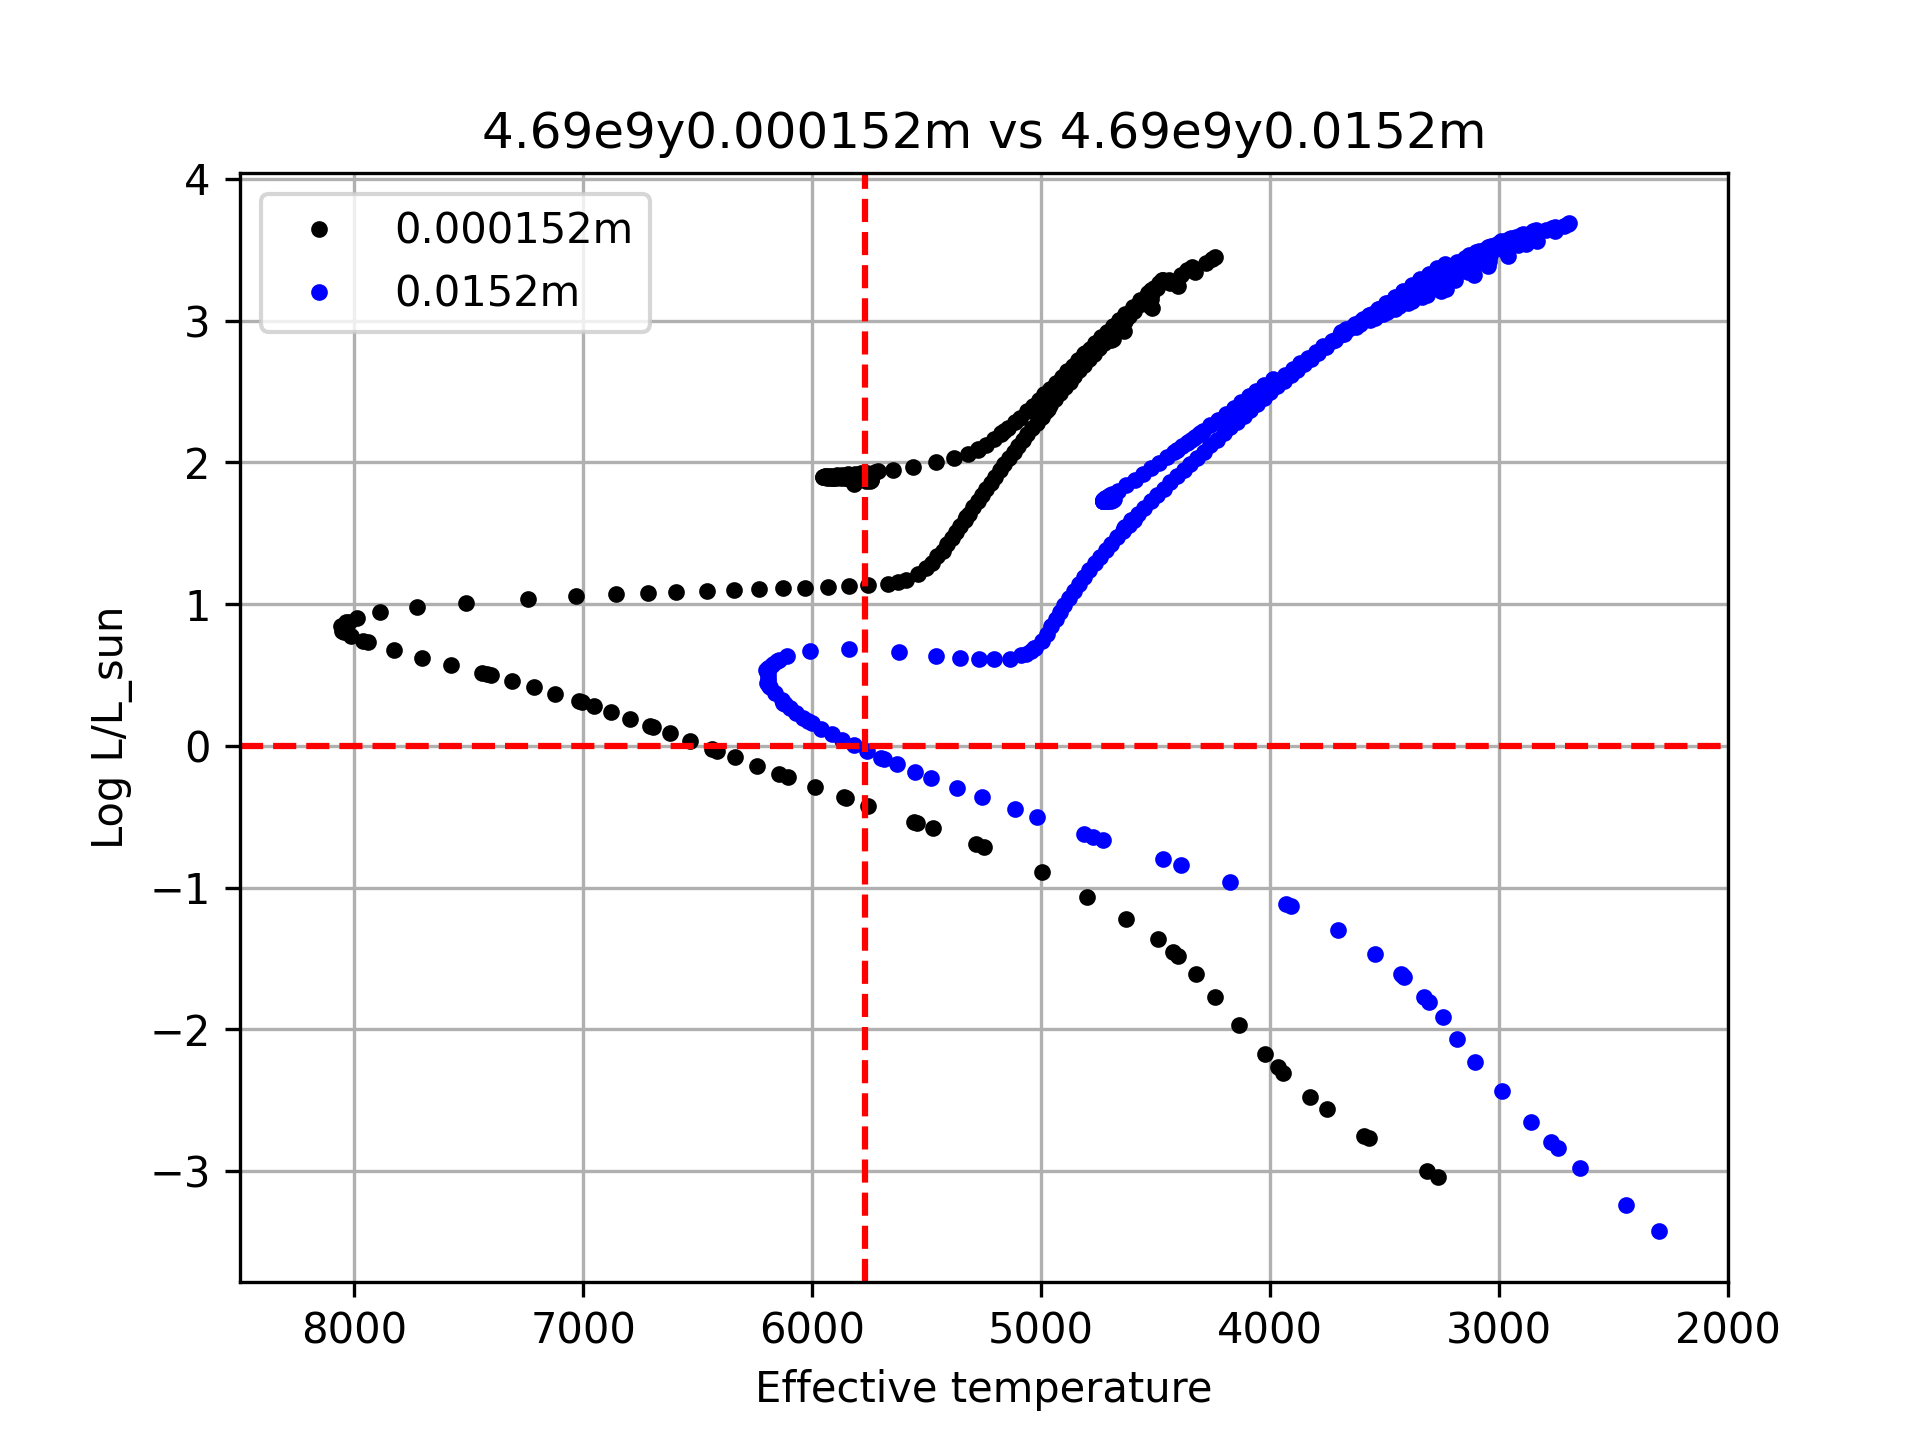
\includegraphics[width=12cm]{figures/0.000152m_vs_0.0152m}
        \label{fig:metallicityComparison}
    \end{figure}

    \textbf{10} \textit{How is this value of 0.75 magnitudes derived? Why do the unresolved binary systems appear as a ``scattering''?}

    Apparent magnitude is defined as (with sun as reference):

    \begin{equation}
        m_x = -5 \cdot \log_{100}{\frac{B_x}{B_\odot}}
        \label{eq:apparentMagDef}
    \end{equation}

    If $B_x$ is the flux from an unresolved binary where the brighter of the constituent stars has flux $B_y$ then $B_x$ will be some multiplier $\lambda \in (1,2]$ times $B_y$, i.e. $B_x = \lambda \cdot B_y$.
    A value of $\lambda = 1$ would correspond to the less bright star in the binary having 0 flux relative to the brighter star.
    Whilst $\lambda = 2$ would correspond to two equally bright stars.
    To find how much an unresolved binary could possibly deviate we'll explore $B_x = 2 B_y$, inserting this into the definition would give us:

    \begin{equation}
        \begin{gathered}
            m_x = -5 \cdot \log_{100}{\frac{B_x}{B_\odot}} = -5 \log_{100}{\frac{2\cdot B_y}{B_\odot}}\\
            = -5 \( \log_{100}{\frac{B_y}{B_\odot}} + \log_{100}{2}\) = -5 \cdot \log_{100}{2} - 5 \cdot \log_{100}{\frac{B_y}{B_\odot}}\\
            = -5 \cdot \log_{100}{2} + m_y \approx 0.75 + m_y
        \end{gathered}\label{eq:derivationBinaryMag}
    \end{equation}

    The peak luminosity of the binary should be at about the wavelenth of peak luminosity of the brighter star.
    Thus the unresolved binary would appear in the HR-diagram around the point on the x-axis where the brighter star would appear on its own but shifted upward.

    How much a binary is shifted upwards depends on the difference in flux between the stars in the binary.
    The smaller the difference is the larger the deviation would be from the main sequence, up to 0.75 if they have the same flux.
    The ''scattering`` comes from the fact that the difference in flux varies between binary systems



\end{document}
